%=========================================================================
% (c) 2011, 2012 Josef Lusticky <xlusti00@stud.fit.vutbr.cz>

\section{Algorithms}
NTP uses the intersection algorithm for selecting the possible most exact timestamp recieved
from various servers. The resulting exact timestamp does not have to be the same
as one of those servers provided.
There are four timestamps in NTP packet: Reference, Origin, Receive and Transmit timestamp.
The 64-bit long NTP format is used for expressing them~\cite{rfc5905}.
Using these four timestamps NTP can compute the
the offset which is given by $\theta = \frac{1}{2}[(t_1 - t_0) + (t_2 - t_1)]$
where $t_0$ is the time of the request packet transmission,
$t_1$ is the time of the request packet reception,
$t_2$ is the time of the response packet transmission and
$t_3$ is the time of the response packet reception~\cite{ntp-algor}.

When computing result from more servers the intersection algorithms is used~\cite{rfc5905}.
First of all a set of bad and good servers must be made.
Bad servers are called Falsetickers and good are called Truechimers~\cite{rfc5905}.
The division to these sets is based on their response.
As one can assume for sensible result there must be more Truechimers than Falsetickers~\cite{rfc5905}.
% TODO f < M\2
Intersection algorithm computes with estimates converted to intervals.
E.g. if we have the estimates $10 \pm 2$, $12 \pm 1$ and $11 \pm 1$
then these intervals are $<8; 12>$, $<11; 13>$ and $<10; 12>$ which
intersect to form $<11; 12>$ or $11.5 \pm 0.5$ as consistent with all three values.
The arithmetic mean is used as a value of result.
When querying servers again the algorithm repeats but the new result computation
also depends on the previous result~\cite{rfc5905}.
This eliminates possible jitter which can be caused by reapeatedly quering the servers
and getting slightly different answers from them.

\begin{figure}
	\centering
	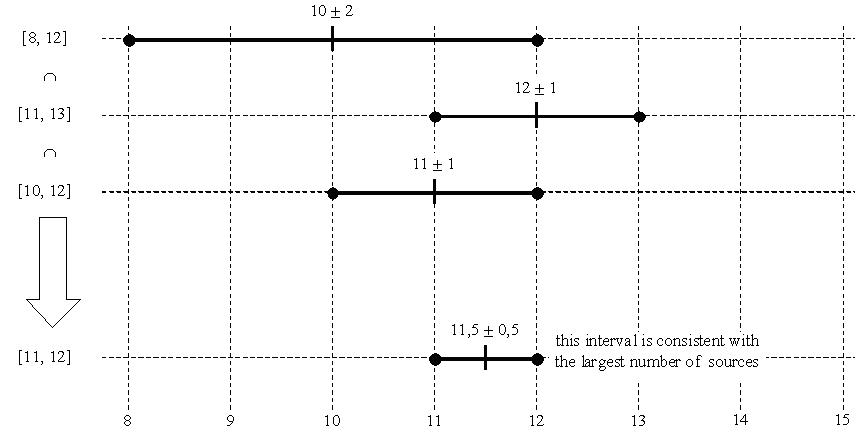
\includegraphics[width=13cm,keepaspectratio]{fig/Marzullo_example-1.jpg}
	\caption{Intersection algorithm}
	\label{fig:ntp-intersection}
	\bigskip
\end{figure}

